
La interfaz de usuario parte de un menú principal del que parten las diversas opciones. Siempre que el usuario cancele una operación o finalice una petición volverá a este menú principal.
La petición de una solicitud de recogida es una secuencia de pasos en los cuáles el usuario indica qué enseres desea que se le recojan, seguidamente facilita el punto de recogida más cercano de donde tiene los enseres (que habitualmente es su domicilio), acto seguido se informa de las condiciones de uso del servicio y de que sus datos de nombre y teléfono quedarán registrado en el sistema acorde con la legislación existente. Ya por último se le confirma la fecha de recogida. Para la enciclopedia únicamente se informa de los tipos de contenedores existentes y la finalidad de cada uno así como los diversos procedimientos para el reciclaje de residuos. Por último se incluye adicionalmente una vista para que el usuario pueda consultar las solicitudes de recogida de enseres que ha realizado anteriormente y las que tiene pendientes de realización. 
% Esquema de vistas de la UI
\begin{figure}[H]
\centering
	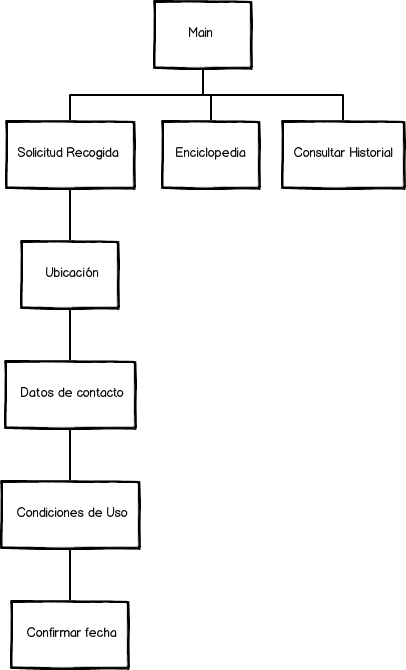
\includegraphics[scale=0.5]{Views.png} 
\caption{Esquema de vistas de la aplicación.}
\end{figure}	

A continuación se incluyen los diversos bocetos de las distintas pantallas de la aplicación móvil. 

% VISTA MENÚ PRINCIPAL
 \begin{figure}[H]
\centering
	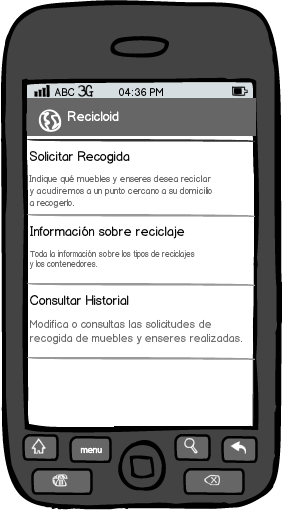
\includegraphics[scale=0.5]{MainLayout.png} 
\caption{Boceto del menú principal}
\end{figure}
Esta es la primera ventana que visualiza el usuario, se incluye el titulo de la aplicación acompañado de un pequeño icono que la identificará en todo momento. Debajo de esta una lista con las 3 opciones principales y cada una de ellas acompañadas de una breve descripción de en qué consiste cada una de ellas. Se incluye además una imagen que identifica visualmente cada opción para mayor comodidad del usuario. Este menú principal puede ir precedido de un \textit{splash} con la imagen de la organización encargaría de prestar el servicio. Una vez se haga \textit{click} sobre alguna de las tres opciones se abrirá la vista correspondiente. 
% VISTA SOLICITUD RECOGIDA
 \begin{figure}[H]
\centering
	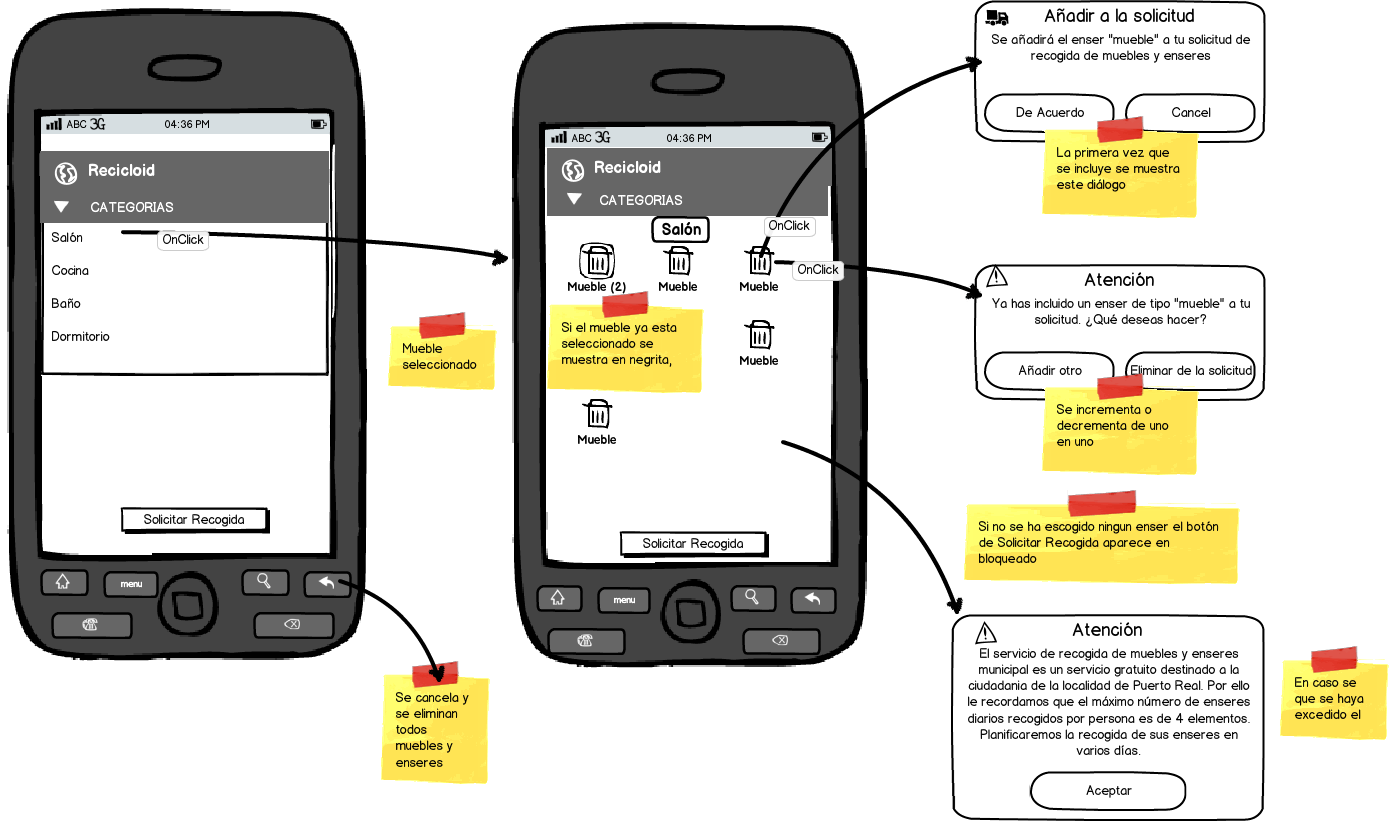
\includegraphics[scale=0.35]{SolicitudRecogidaLayout.png} 
\caption{Boceto de la solicitud de recogida}
\end{figure}
Una vez el usuario ha seleccionado la opción de solicitar recogida, se muestra un menú desplegable con todas las categorías existentes (se categorizan los muebles y enseres en función de su ubicación). Una vez el usuario selecciona en el menú desplegable una habitación se muestra una ventana con pequeños iconos acompañados de texto con los distintos muebles y enseres que corresponden a dicha habitación. Cuando el usuario hace click en uno por primera vez se haber una ventana emergente en la cual se informa al usuario que dicho enser será añadido al listado de muebles y enseres de la solicitud, se pide confirmación o cancelación. Si el usuario indica que desea añadirlo éste queda resaltado y con el texto en negrita. Además el texto aparece acompañado con un paréntesis donde se indica la cantidad de enseres que se han seleccionado. \\
Si el usuario marca por segunda vez un icono de enser que ya ha sido previamente seleccionado aparece una nueva ventana emergente que posibilita incrementar el enser en uno, o bien eliminar todos los enseres de ese tipo de la solicitud. \\
En caso de que el usuario añada un cuarto enser a su solicitud se informa al usuario de que su petición se llevará a cabo en varios días, ya que el máximo diario establecido por usuario es de la recogida de 4 enseres al día. También se controla que el usuario no ejecuté solicitudes vacías demarcando el botón hasta que se escoja al menos un mueble y enser. En caso de que el usuario seleccione volver al menú principal se eliminan todos los iconos marcados y se deja como inicialmente encontraba. 
% UBICACIÓN
 \begin{figure}[H]
\centering
	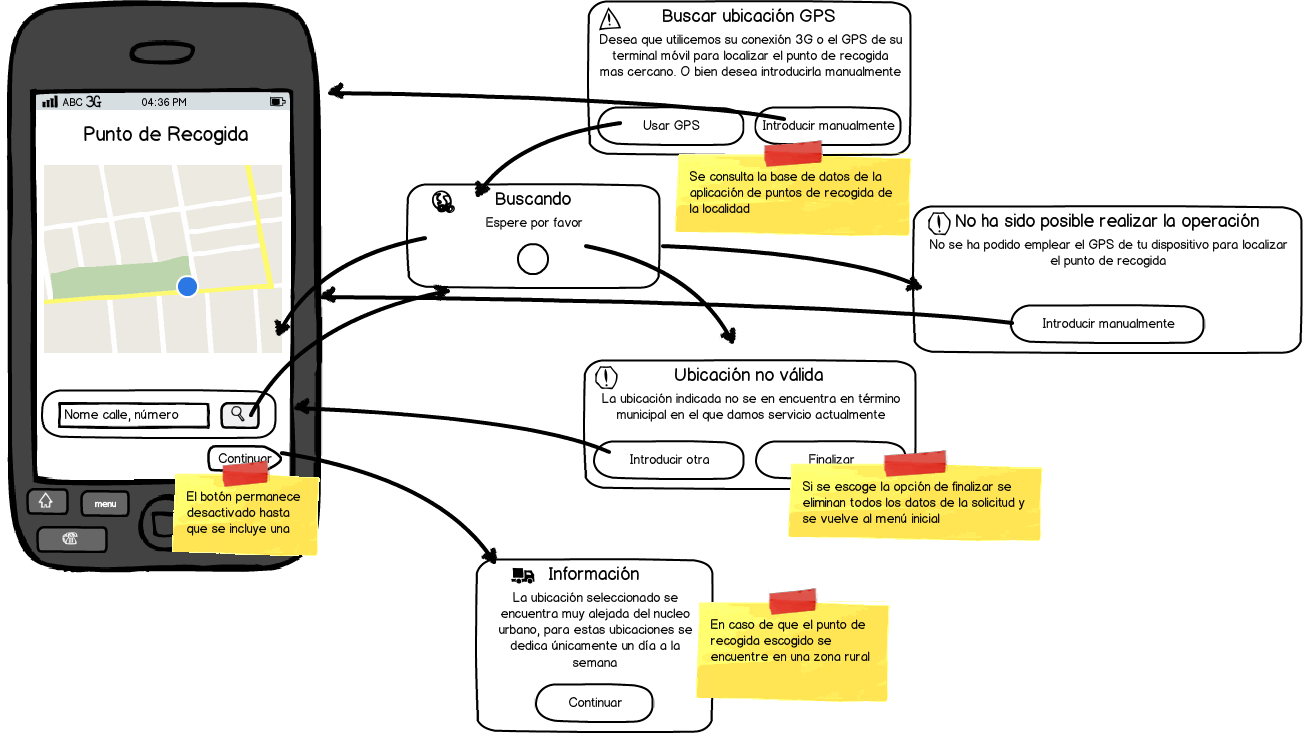
\includegraphics[scale=0.35]{SolicitudUbicacionLayout.png} 
\caption{Boceto de ubicación de la recogida}
\end{figure}
Se muestra una ventana al usuario preguntándole si desea que se localice el punto mas cercano del que se encuentra actualmente haciendo uso del dispositivo móvil, o bien si desea introducirla manualmente \\
En caso de escoger la opción de \"Usar GPS" se hará uso de la tecnología existente en el terminal móvil para obtener la ubicación actual y seguidamente contrastarlo con la base de datos local del teléfono móvil con todos los puntos de recogidas existentes. Si se localiza correctamente se muestra en el mapa y se indica el nombre del a calle y el número más cercano. Puede ocurrir que la ubicación se encuentre fuera del termino municipal donde se preste servicio en cuyo caso se mostrará un mensaje informando de que la ubicación no es válida y posibilitando que introduzca manualmente una nueva ubicación. De igual manera, pude ocurrir que el dispositivo GPS no funcione correctamente en cuyo caso se informará del error y se indicará al usuario que introduzca manualmente la dirección. Durante la duración de la operación de búsqueda en el dispositivo GPS aparecerá una ventana de cargando con una animación y un mensaje solicitando al usuario su espera. Se establecerá un tiempo máximo de respuesta.  \\
Si el usuario escoge introducir manualmente su ubicación introducirá su calle y su número. Posteriormente el sistema detectará las coordenadas del domicilio del cliente y buscará la ubicación más cercana cotejando con la base de datos de puntos de recogida existente en el sistema. De igual manera puede darse el caso de que la ubicación no sea válida al encontrarse fuera del término municipal.  \\
Finalmente una vez obtenida la dirección del punto de recogida en el caso de que el punto de recogida esté alejado del término municipal se informa al usuario de las condiciones de uso existentes para esta tipología de usuarios.  \\
El botón para continuar con el proceso de solicitud de recogida de muebles y enseres no estará habilitado hasta que se haya escogido un punto de recogido válido. 

% DATOS DE CONTACTO
 \begin{figure}[H]
\centering
	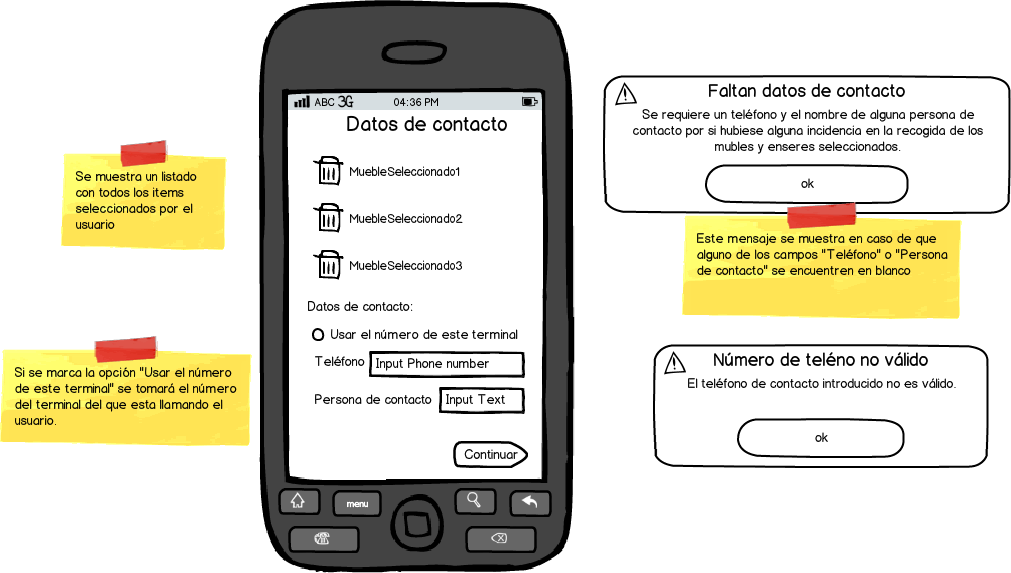
\includegraphics[scale=0.35]{SolicitudDatosContactoLayout.png} 
\caption{Boceto de datos de contacto}
\end{figure}
Se muestra una ventana en la que solicitan al usuario sus datos de contacto, en la parte superior a modo de recordatorio se incluye un listado de todos los enseres que ha solicitado el usuario que sean recogidos. Debajo de estos se muestra un formulario en el que se piden al usuario sus datos de contacto. Estos datos pueden ser introducidos manualmente por el usuario o bien ser tomados del propio terminal móvil. Se comprueba que el número de teléfono es correcto y que ambos cambios han sido rellenado correctamente antes de continuar con el proceso de tramitación de la solicitud. 

% CONDICIONES DE USO
 \begin{figure}[H]
\centering
	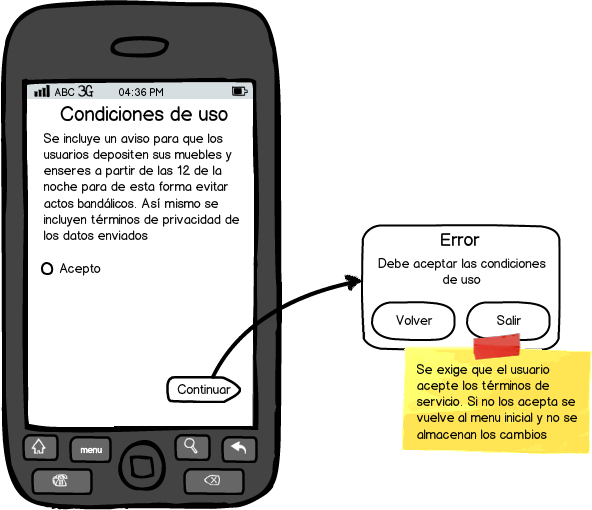
\includegraphics[scale=0.35]{SolicitudCondicionesLayout.png} 
\caption{Boceto de las condiciona de uso}
\end{figure}
Antes de finalizar el proceso y dado que los datos del usuario quedarán registrados en el servidor se muestra una ventana con las condiciones de uso y aspectos legales. Entre estas condiciones están las requeridas por la organización de informar a los usuarios de su responsabilidad de despistar los muebles y enseres a la hora mas tardía de la noche posible para evitar posibles actos vandálicos así como información referente al uso de sus datos por parte de la organización. El usuario debe aceptar las condiciones de uso para hacer uso del servicio.

% FECHA DE RECOGIDA
  \begin{figure}[H]
\centering
	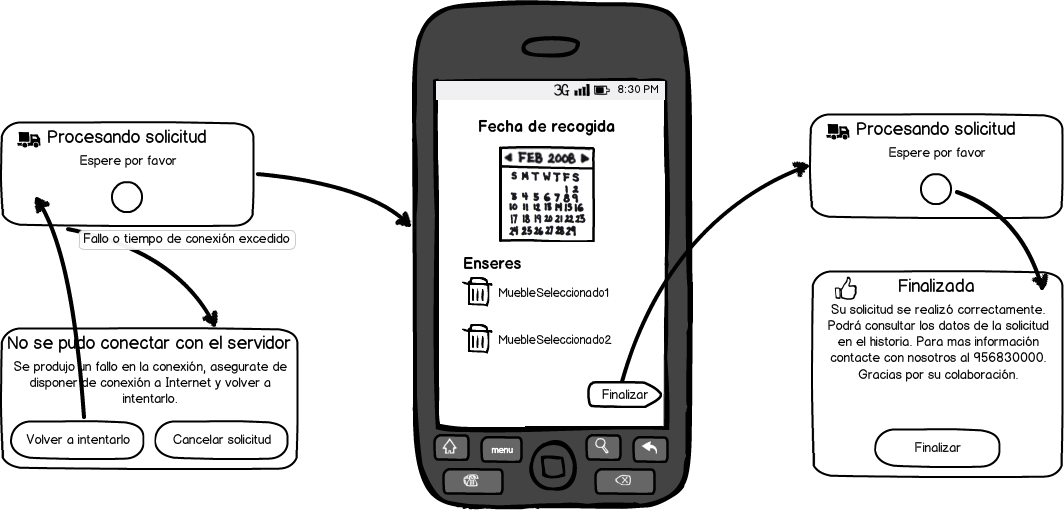
\includegraphics[scale=0.35]{SolicitudFechaLayout.png} 
\caption{Boceto de fecha de recogida}
\end{figure}
Se establece una conexión con el servidor para concertar la fecha de la recogida de muebles y enseres. En caso de producirse un error o de no tener habilitada la conexión se mostrará una ventana emergente con el error que se ha producido para que el usuario reintente la conexión o bien cancele el proceso. Una vez establecida la conexión se muestra un calendario con las fechas establecidas  y un recordatorio con los enseres que serán depositados. En el caso de ser mas de 4 enseres aparecerán varias fechas remarcadas en el calendario. Una vez el usuario confirma las fechas se establece una segunda conexión en la que se confirma la solicitud mediante un mensaje de agradecimiento al usuario y un recordatorio del teléfono de contacto para cualquier duda posible. Finalizado el proceso se vuelve al menú principal. 

% ENCICLOPEDIA DE RECICLAJE
  \begin{figure}[H]
\centering
	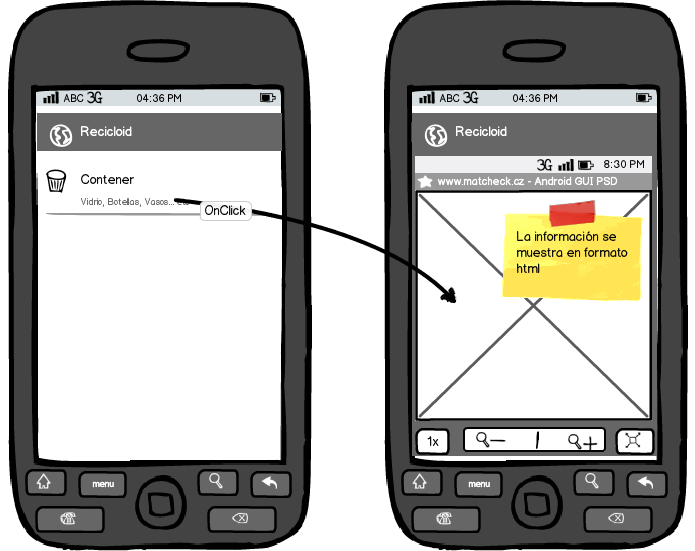
\includegraphics[scale=0.35]{EnciclopediaLayout.png} 
\caption{Boceto de guía de reciclaje}
\end{figure}
La aplicación incluye una guía de reciclaje en la que se muestran los distintos tipos de contenedores y un breve resumen del tipo de residuos que van depositados en dicho contenedor. Si el usuario marca alguno de los contenedores se abre el navegador web del usuario a una página en formato adaptado para terminales móviles con información sobre dicho tipo de contenedor un listado del tipo de residuos que van en dicho contenedor. Esta web funciona a modo local y no requiere de conexión a internet.

% HISTORIAL 
  \begin{figure}[H]
\centering
	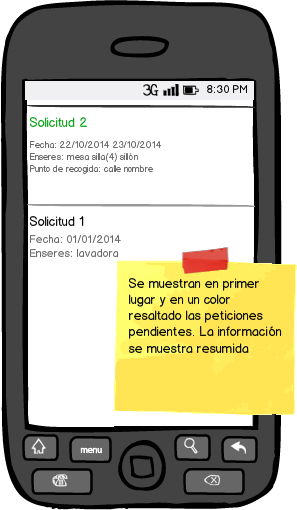
\includegraphics[scale=0.35]{HistorialSolicitud.png} 
\caption{Boceto de historial de solicitudes}
\end{figure}
La tercera de las opciones del menú principal es el \textit{Historial de solicitudes}. Mediante esta opción se muestra al usuario un listado resumido de las solicitudes que se han realizado. En primer lugar aparecerán resaltado en verde las que se han realizado para días posteriores a la fecha del sistema. Debajo de ésta aparecerán las peticiones cursadas anteriormente y cuya fecha de recogida ya ha transcurrido. \\
